A standard method for computing the Tucker decomposition is the Higher-Order SVD 
(\hosvd)~\cite{Lathauwer00amultilinear}, a generalization of the singular value 
decomposition to tensors.
% 
As mentioned in~\cref{sec:hosvd}, a direct approach to the \hosvd involves computing a series of SVDs of 
unfolded tensors to compute the orthogonal factor matrices whose 
columns approximately span the columns of the unfolded tensor (i.e., the 
mode-$k$ fiber space). We will refer to this computation as the Mode-wise Truncated Fiber Space Basis Computation (\MTFSBC).
Following this operation, the resulting factor matrices are applied to the input tensor to compress the original data.
%

%
We consider a distributed-memory application for large dense tensors, as might arise in large-scale 
scientific simulations. For instance, we consider a five-way tensor representing three spatial dimensions, 
a time dimension, and a number of different variables. A user may wish to examine this data on a local 
machine with limited memory or to store many simulations in limited storage, and the \hosvd has been 
shown to be a highly scalable method for performing this compression.
The current state of the art for distributed \hosvd is TuckerMPI\footnote{\url{http://tensors.gitlab.io/TuckerMPI/}}, 
based on the work of Austin, Ballard, and Kolda~\cite{AuBaKo16}. As in the Gram approach of~\cref{sec:hosvd}, the \MTFSBC kernel is performed with a distributed Gram matrix computation followed by a local eigensolve. The factors are then applied to the input tensor using a distributed tensor-matrix multiplication, forming the dense core tensor. The core tensor and factor matrices can be used to construct an approximation to the original data or any subset thereof.

\paragraph{Distributed implementation}
% \TODO{Suggest $\ell$ rather than $q$ as processor index.}
We will assume the tensor is distributed according to a \emph{Cartesian} distribution.
Given a processor grid $p_1 \times \cdots \times p_d$, we define notation such that the total number of processors
is $p^d = \prod_{k=1}^d p_k$. We use an overbar to denote a local object,
so each process owns a tensor $\bar{\T{X}}$ which is a subtensor of $\T{X}$.
Assuming for 
notational convenience that $n_k$ evenly divides $p_k$, the size of each subtensor 
is $\frac{n_1}{p_1} \times \cdots \times \frac{n_d}{p_d}$, so process $(\ell_1,\dots,\ell_d)$ 
owns the subtensor  with range $\mathbf{i} = ((\ell_1-1)\frac{n_1}{p_1}:\ell_1\frac{n_1}{p_1}-1,\dots)$. 
Furthermore, if we matricize a subtensor in mode $k$ to produce $\bar{\M{X}}_{(k)}$, 
the result is a submatrix in the full matricization $\M{X}_{(k)}$. 
This is visualized in~\cref{fig:tensor_block_dist}, though the columns owned by a processor are not always contiguous as shown here.
Collective communications in this 
model are then implemented either on block-rows or block-columns. 

The column-communicator for process $(\ell_1,\dots,\ell_d)$ in mode $k$ is the set of $p_k$ 
processes $(\ell_1,\dots,\ell_{k-1},*,\ell_{k+1},\dots,\ell_d)$, whereas the row-communicator is 
the set of $p_k^\oslash$ processes $(*,\dots,*,\ell_k,*,\dots,*)$. 
These communicators are visualized in~\cref{fig:tensor_comm}.
% \begin{figure}[]
  \centering
  \begin{tikzpicture}[scale=.3,textnode/.style={scale=.6}]
    \def\ix{3} %
    \def\iy{4} %
    \def\iz{2} %
    \def\sx{1.5} %
    \def\sy{1}
    \def\sz{2}
    \def\offset{0.25}
    \def\myquad{0.5}
    \draw (0,0) grid[xscale=\sx,yscale=\sy] (\ix,\iy); %
    \node[textnode,below] at (0.5*\ix*\sx,0) {$\leftarrow \; n_2 \; \rightarrow$};
    \node[textnode,rotate=90,above] at (0, 0.5*\iy*\sy)  {$\leftarrow \; n_1 \; \rightarrow$};
    \begin{scope}[shift={(XFrontLowerLeft)},canvas is zx plane at y=\iy*\sy,rotate=90]
      \draw (0,0) grid[xscale=\sx,yscale=\sz] (\ix,\iz); %
    \end{scope}
    \begin{scope}[shift={(XFrontLowerLeft)},canvas is zy plane at x=\ix*\sx,rotate=90]
      \draw (0,0) grid[xscale=\sy,yscale=\sz] (\iy,\iz); %
      \node[textnode,rotate=45,below] at (0,0.5*\iz*\sz) {$\leftarrow \; n_3 \; \rightarrow$};
    \end{scope}
  \end{tikzpicture}
  \caption{Tensor  on $4 {\times} 3 {\times} 2$ processor grid.}
  \label{fig:tensor_block_dist}
\end{figure}
\begin{figure}
  \centering 
  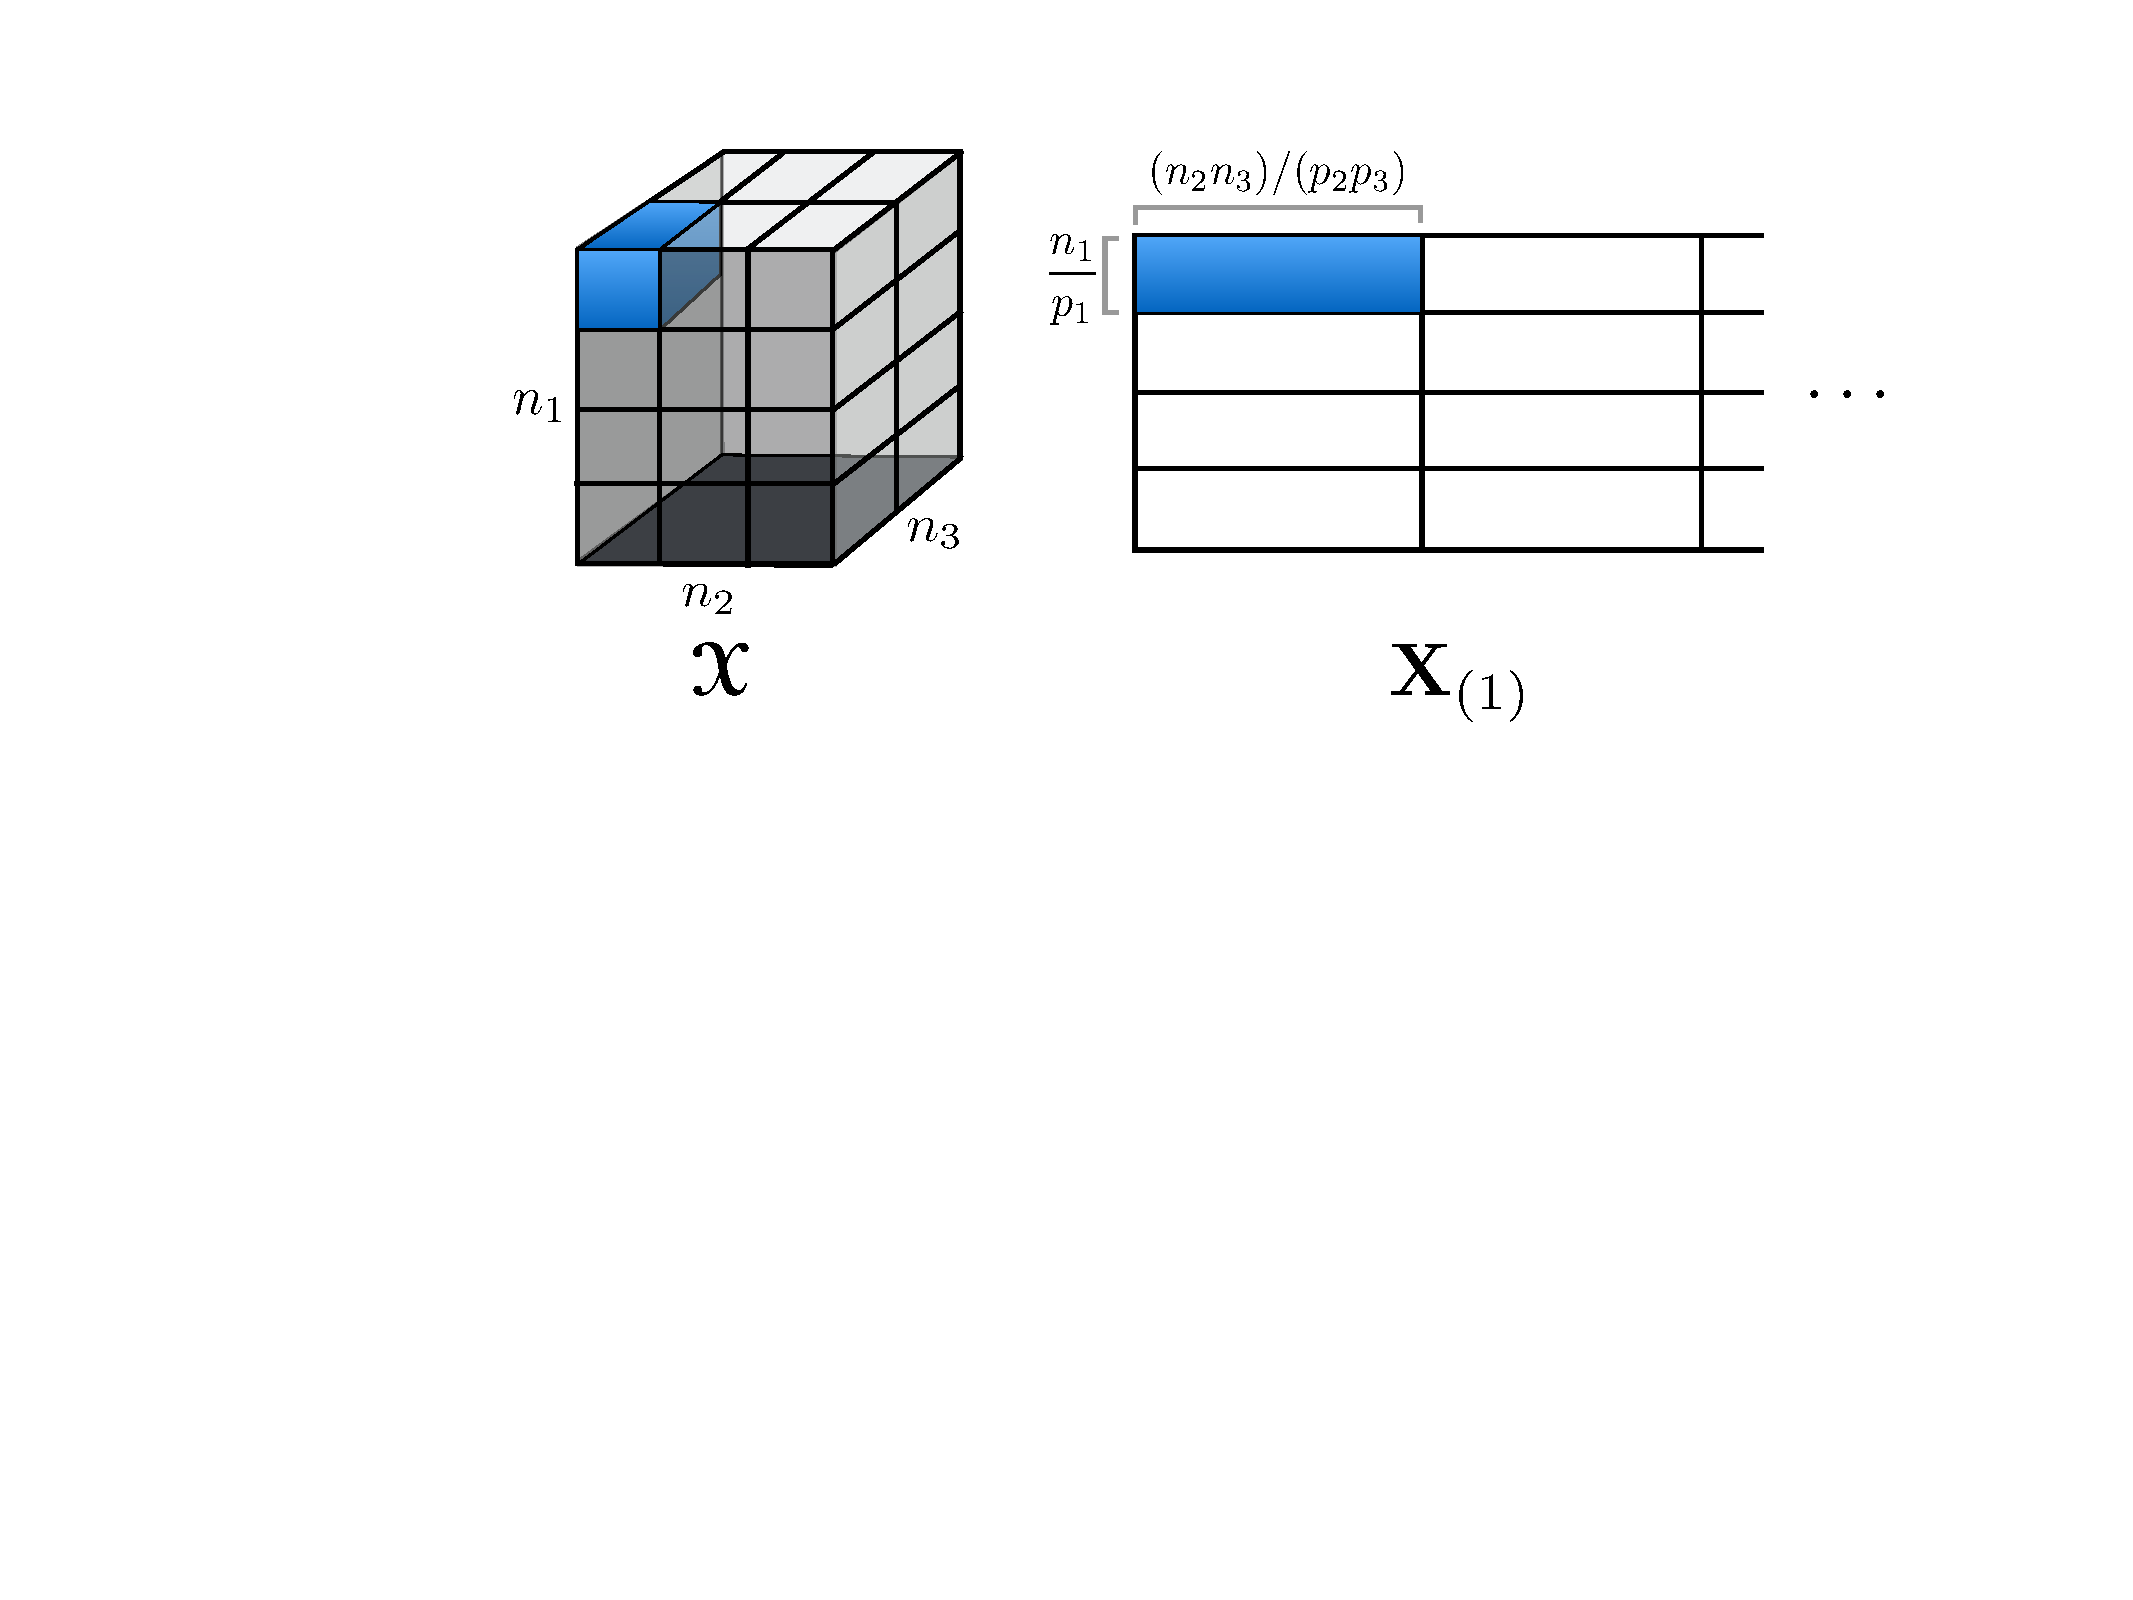
\includegraphics[width=0.6\linewidth]{figs/cartesian}
  \caption{A tensor on a $4\times3\times2$ processor grid. The matricized subtensor shown in blue maps to a submatrix in the distributed matricized tensor, as illustrated on the right. 
  %\GB{I'm changing ``block'' to ``submatrix'' because it's not necessarily a contiguous block if you unfold in a middle dimension (the rows are contiguous but the columns may not be).}
  }
  \label{fig:tensor_block_dist}
\end{figure}
\begin{figure}
  \centering 
  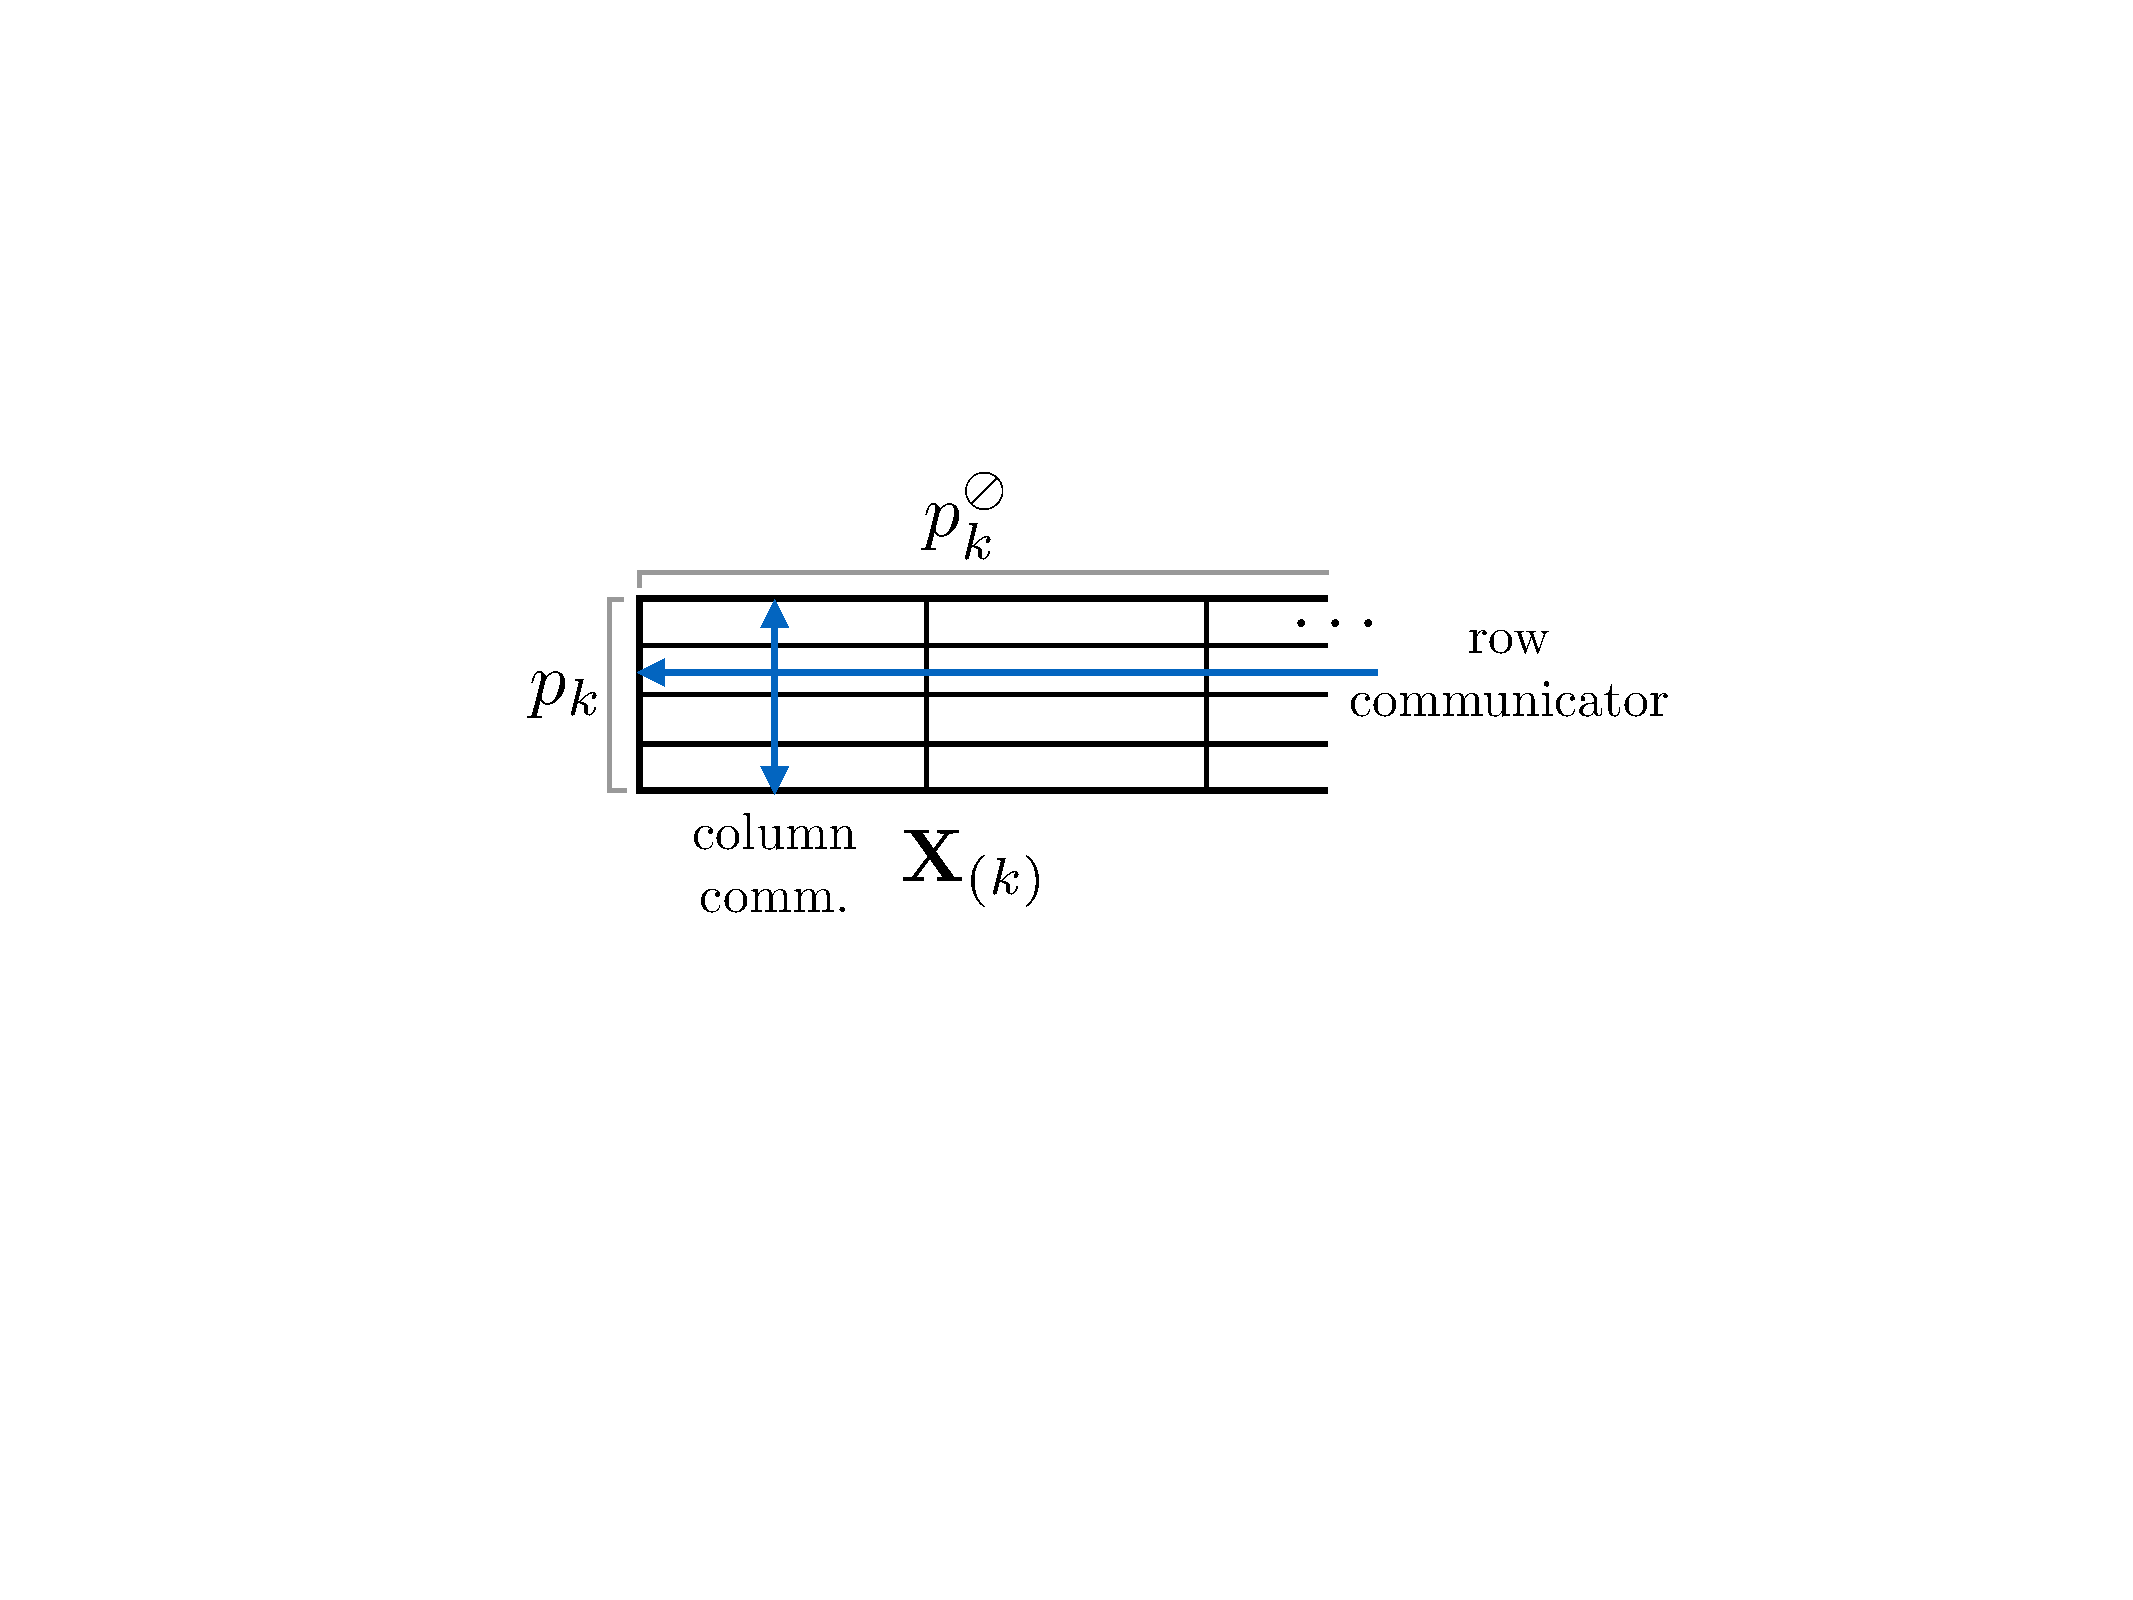
\includegraphics[width=0.55\linewidth]{figs/communicators}
  \caption{A process-centric view of~\cref{fig:tensor_block_dist}. The column-communicator in mode $k$ is the set of $p_k$ processes that own blocks in the same column of $\M{X}_{(k)}$, while the row-communicator is the set of $p_k^\oslash$ processes that own blocks in the same row.}
  \label{fig:tensor_comm}
\end{figure}

\paragraph{Proposal}
We propose efficiently performing the \MTFSBC kernel in distributed memory by applying methods 
from randomized numerical linear algebra. We propose that a series of local multiplications followed by a small 
global communication can result in a \emph{sketch} of the original tensor that fits in local memory. 
% with comparable error. 
% Though randomized methods work with only a subset of the data, the errors are very close.
Finally, we propose to apply this to the efficient computation of a Tucker decomposition for the compression of scientific data.
%The following is a more detailed breakdown of our contributions:
%Using this sketch we can, with the help of our theoretical results, compute an \hosvd that still satisfies (with high probability) the error tolerance. 
% \TODO{Include a plot of compression ratio / speed between TuckerMPI and sketching method.}
We summarize our proposed contributions as follows:
\begin{itemize}
  \item Implement and develop a cost analysis for an efficient sketch-based \MTFSBC in 
  distributed memory, using randomization to reduce computation and communication. This method would exploit the Kronecker structure of the sketching operation to reduce computation.
  \item Introduce a new parallel method for a sequence of tensor-times-matrix operations that trades extra computation for reduced communication and show how and when this can be used to further increase the efficiency of sketching. 
  \item Apply our kernel to the Tucker tensor decomposition, benchmark our method on large-scale scientific 
  data sets, and demonstrate scaling on synthetic data sets to improve upon the fastest known 
  traditional implementation.
  \item Provide theory to show how the error introduced through randomization can be compensated for.
  % No previous work has considered this issue, but it is key to preserving data accuracy.
\end{itemize}

\paragraph{Sketching as a series of TTMs}
Consider the algorithm for estimating the range of a matrix in~\cref{alg:rrf}. 
Similarly, to estimate the range of an unfolded tensor we can compute
$\M{Y}_{(k)} \gets \M{X}_{(k)} \M{\Omega}$, where $\M{\Omega}$ 
is a $n_k^\oslash \times \ell$ random matrix. This approach has previously been taken for tensors~\cite{bigtens,DBLP:conf/acssc/VervlietDL16,Navasca2015}. The cost of this step would be 
comparable to a TTM, which could easily become a bottleneck.
However, suppose instead that we multiply with a \emph{Kronecker} product of $d-1$ small random matrices of size $s_k \times n_k$:
\begin{equation}
  \label{eqn:sketchasgemm}
  \M{Y}_{(k)} \gets \M{X}_{(k)} \Big( \M{\Omega}_1 \otimes \cdots \otimes \M{\Omega}_{k-1} \otimes \M{\Omega}_{k+1} \otimes \dots \otimes \M{\Omega}_d \Big)^\trans
\end{equation}
Using~\cref{eqn:ttensor}, we can see that this is equivalent
to performing a series of TTMs with these small matrices:
\begin{equation}
  \label{eqn:sketchasttm}
  \T{Y} \gets \T{X} \times \Big\{ \M{\Omega}_j^\trans \Big\}_{j \neq k}.
\end{equation}

We propose to use this method because it uses far fewer flops than previous work, and the operation can be efficiently performed in distributed memory as a series of distributed TTMs. 

\paragraph{Reducing communication of a TTM sequence}
We present a novel method for computing a TTM sequence in distributed memory which outperforms standard methods when the input matrices have a large aspect ratio (so that the output tensor is much smaller than the input tensor). 
This method significantly reduces communication in certain cases but may be more expensive in others.
It also performs more computation than the standard approach, so we use a performance model to guide its usage.

Consider computing a sequence of TTMs $\T{Y} \gets \T{X} \times_1 \M{A} \times_2 \M{B} \times_3 \M{C}$. Previous implementations of the TTM~\cite{AuBaKo16} first perform the local multiply $\bar{\M{A}}\bar{\M{X}}_{(1)}$ on each process, forming an intermediate result of size $s_1 \times n_1^\oslash / p_1^\oslash$. This is followed by a Reduce-Scatter among the column communicator so that each process owns a local result of size $s_1/p_1 \times n_1^\oslash / p_1^\oslash$, and the process is repeated for the following modes $k=2$ and $k=3$. 
If the matrices $\M{A}$, $\M{B}$, and $\M{C}$ have more columns than rows, then the tensor gets smaller at each step.
While this standard method is work efficient, it involves communicating the intermediate tensors in each step, which are larger than the final output.

We propose that this communication can be \emph{deferred} until later steps, while still maintaining the correct output. We will call this proposed deferred-communication approach \emph{\dTTM}, noting that element $(i,j,k)$ of $\T{Y}$
can be written element-wise using~\cref{eqn:contractionelem} as
\begin{equation}
  \label{eqn:elemwisemttm}
  y_{ijk} = \sum_\mu \sum_\nu \sum_\xi x_{\mu \nu \xi}a_{\mu i}b_{\nu j}c_{\xi k}.
\end{equation}

While this approach isn't work optimal, the reduction in communication should yield useful applications, particularly for low-flop operations such as sketching. We propose to elaborate on this communication/computation tradeoff.